 
\subsection{Experiment setup}

We implement the benchmarks on Google Cloud, which is a mainstream cloud platform to provide serverless functions. 
For local measurements, we use an Ubuntu 20.04-64bit machine with Intel(R) Core(TM) i7-8750H CPU @ 2.20GHz processor and 12GB RAM.
We plan to do experiments in more types of machines and operating systems to show the generality of the benchmark.

%\subsection{Factors impacting context switches in serverless environment}
% TODO

\subsection{Measuring local context switches}

All the previous benchmarks\cite{cs-web,cs-datasize,cs-lmbench,cs-pipes} are implemented in C language.
However, currently Google Cloud only supports functions written in Node.js, Go, Java, Python and Ruby.
Considering that Python is one of the most popular languages, rewriting the prior benchmarks in Python and examining its correctness in local PC is important.

The context switch time measured by the first three benchmarks in local PC is usually among 2us from Table~\ref{tab:experiment1}.
In the first row, pipe, condition var and lmbench refers to methods listed in Section 2 respectively.
However, when it's rewritten by Python, the measured time is 10 times larger than previous results. 
The reason might be that extra execution is added to the time measurement when translating the language.
What's more, the C programs execute faster as compiled programs while Python executes slower due its interpreted programs, 
and these extra execution time is more obvious when using python. 
Therefore, we plan to measure the time variation induced by Python on local computers and scale the measured time in cloud accordingly.
Table~\ref{tab:experiment1} shows that the context switch time measured by the pipe method written in Python is about 17.14 times larger than measuring in C programs.
In our further experiment in cloud, we'll take the python measured time divided by 17.14 as the context switch time.

\subsection{Measuring context switches in the cloud}

We create functions with different memory allocated and measure the context switch time with the Ping pong pipes method.
For each memory configuration we run 10 times and get the average of the calculated time. 
We also notion that the variation induced by Python language has already been considered and the value shown in Table~\ref{tab:cloud} is processed.
We notice that if the allocate memory is 128GB, the context switch time is remarkably higher than the other configurations.
And we plan to look deeper into this in the future.

\begin{center}
    \begin{table}
    \begin{tabular}{||c c c c c||} 
     \hline
     Benchmark & Pingpong& Condition Var & Lmbench & Pipe(python) \\ 
     \hline
     Time(/us) & 1.96 & 2.29 & 1.78 & 33.6\\ 
     \hline
    \end{tabular}
    \caption{\label{tab:experiment1}Context switch time by different benchmarks}
\end{table}
\end{center}

\begin{center}
    \begin{table}
    \begin{tabular}{||c c c c||} 
     \hline
      Memory(/MB) & 128 & 256 & 512 \\ 
     \hline
     Time(/us) & 81.11 & 33.96 & 36.17 \\ 
     \hline
    \end{tabular}
    \caption{\label{tab:cloud}Context switch time in functions with different memories }
\end{table} 
\end{center}
% Figure~\ref{fig:attack-1}.

% \begin{figure}
% 	\centering
% 	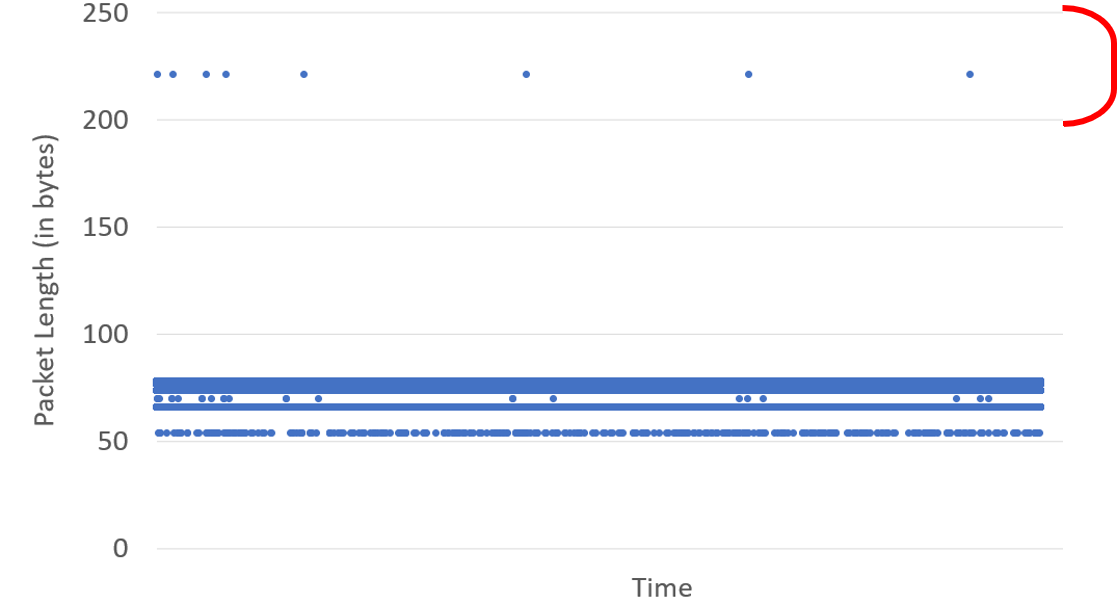
\includegraphics[width=\linewidth]{figure/attack1.png}
% 	\caption{Plot of Modbus packet lengths}
% 	\label{fig:attack-1}
% \end{figure}
